\documentclass[10pt]{article}

%%%%%%%%%%%%%%%%%%%%%%%%%%%%%%%%%%%%%%%%%%%%%%%%%%%%%%%%%%%%%%%%%%%%%%%%%%%%%%%%
% LaTeX Imports
%%%%%%%%%%%%%%%%%%%%%%%%%%%%%%%%%%%%%%%%%%%%%%%%%%%%%%%%%%%%%%%%%%%%%%%%%%%%%%%%
\usepackage{amsfonts}                                                   % Math fonts
\usepackage{amsmath}                                                    % Math formatting
\usepackage{amssymb}                                                    % Math formatting
\usepackage{amsthm}                                                     % Math Theorems
\usepackage{arydshln}                                                   % Dashed hlines
\usepackage{attachfile}                                                 % AttachFiles
\usepackage{cancel}                                                     % Cancelled math
\usepackage{caption}                                                    % Figure captioning
\usepackage{color}                                                      % Nice Colors
\input{./lib/dragon.inp}                                                % Tikz dragon curve
\usepackage[ampersand]{easylist}                                        % Easy lists
\usepackage{fancyhdr}                                                   % Fancy Header
\usepackage[T1]{fontenc}                                                % Specific font-encoding
%\usepackage[margin=1in, marginparwidth=2cm, marginparsep=2cm]{geometry} % Margins
\usepackage{graphicx}                                                   % Include images
\usepackage{hyperref}                                                   % Referencing
\usepackage[none]{hyphenat}                                             % Don't allow hyphenation
\usepackage{lipsum}                                                     % Lorem Ipsum Dummy Text
\usepackage{listings}                                                   % Code display
\usepackage{marginnote}                                                 % Notes in the margin
\usepackage{microtype}                                                  % Niceness
\usepackage{lib/minted}                                                 % Code display
\usepackage{multirow}                                                   % Multirow tables
\usepackage{pdfpages}                                                   % Include pdfs
\usepackage{pgfplots}                                                   % Create Pictures
\usepackage{rotating}                                                   % Figure rotation
\usepackage{setspace}                                                   % Allow double spacing
\usepackage{subcaption}                                                 % Figure captioning
\usepackage{tikz}                                                       % Create Pictures
\usepackage{tocloft}                                                    % List of Equations
%%%%%%%%%%%%%%%%%%%%%%%%%%%%%%%%%%%%%%%%%%%%%%%%%%%%%%%%%%%%%%%%%%%%%%%%%%%%%%%%
% Package Setup
%%%%%%%%%%%%%%%%%%%%%%%%%%%%%%%%%%%%%%%%%%%%%%%%%%%%%%%%%%%%%%%%%%%%%%%%%%%%%%%%
\hypersetup{%                                                           % Setup linking
    colorlinks=true,
    linkcolor=black,
    citecolor=black,
    filecolor=black,
    urlcolor=black,
}
\RequirePackage[l2tabu, orthodox]{nag}                                  % Nag about bad syntax
\renewcommand*\thesection{\arabic{section} }                             % Reset numbering
\renewcommand{\theFancyVerbLine}{ {\arabic{FancyVerbLine} } }              % Needed for code display
\renewcommand{\footrulewidth}{0.4pt}                                    % Footer hline
\setcounter{secnumdepth}{3}                                             % Include subsubsections in numbering
\setcounter{tocdepth}{3}                                                % Include subsubsections in toc
%%%%%%%%%%%%%%%%%%%%%%%%%%%%%%%%%%%%%%%%%%%%%%%%%%%%%%%%%%%%%%%%%%%%%%%%%%%%%%%%
% Custom commands
%%%%%%%%%%%%%%%%%%%%%%%%%%%%%%%%%%%%%%%%%%%%%%%%%%%%%%%%%%%%%%%%%%%%%%%%%%%%%%%%
\newcommand{\nvec}[1]{\left\langle #1 \right\rangle}                    %  Easy to use vector
\newcommand{\ma}[0]{\mathbf{A} }                                         %  Easy to use vector
\newcommand{\mb}[0]{\mathbf{B} }                                         %  Easy to use vector
\newcommand{\abs}[1]{\left\lvert #1 \right\rvert}                       %  Easy to use abs
\newcommand{\pren}[1]{\left( #1 \right)}                                %  Big parens
\let\oldvec\vec
\renewcommand{\vec}[1]{\oldvec{\mathbf{#1} } }                            %  Vector Styling
\newtheorem{thm}{Theorem}                                               %  Define the theorem name
\newtheorem{definition}{Definition}                                     %  Define the definition name
\definecolor{bg}{rgb}{0.95,0.95,0.95}
\newcommand{\java}[4]{\vspace{10pt}\inputminted[firstline=#2,
                                 lastline=#3,
                                 firstnumber=#2,
                                 gobble=#4,
                                 frame=single,
                                 label=#1,
                                 bgcolor=bg,
                                 linenos]{java}{#1} }
\newcommand{\python}[4]{\vspace{10pt}\inputminted[firstline=#2,
                                 lastline=#3,
                                 firstnumber=#2,
                                 gobble=#4,
                                 frame=single,
                                 label=#1,
                                 bgcolor=bg,
                                 linenos]{python}{#1} }
\newcommand{\js}[4]{\vspace{10pt}\inputminted[firstline=#2,
                                 lastline=#3,
                                 firstnumber=#2,
                                 gobble=#4,
                                 frame=single,
                                 label=#1,
                                 bgcolor=bg,
                                 linenos]{js}{#1} }
%%%%%%%%%%%%%%%%%%%%%%%%%%%%%%%%%%%%%%%%%%%%%%%%%%%%%%%%%%%%%%%%%%%%%%%%%%%%%%%%
% Beginning of document items - headers, title, toc, etc...
%%%%%%%%%%%%%%%%%%%%%%%%%%%%%%%%%%%%%%%%%%%%%%%%%%%%%%%%%%%%%%%%%%%%%%%%%%%%%%%%
\pagestyle{fancy}                                                       %  Establishes that the headers will be defined
\fancyhead[LE,LO]{Computer Systems Notes}                                  %  Adds header to left
\fancyhead[RE,RO]{Zoe Farmer}                                       %  Adds header to right
\cfoot{ \thepage }
\lfoot{CSCI 2400}
\rfoot{Han}
\title{Computer Systems Notes}
\author{Zoe Farmer}

%%%%%%%%%%%%%%%%%%%%%%%%%%%%%%%%%%%%%%%%%%%%%%%%%%%%%%%%%%%%%%%%%%%%%%%%%%%%%%%%
% Beginning of document items - headers, title, toc, etc...
%%%%%%%%%%%%%%%%%%%%%%%%%%%%%%%%%%%%%%%%%%%%%%%%%%%%%%%%%%%%%%%%%%%%%%%%%%%%%%%%
\pagestyle{fancy}                                                       %  Establishes that the headers will be defined
\fancyhead[LE,LO]{Homework 1}                                  %  Adds header to left
\fancyhead[RE,RO]{Zoe Farmer}                                       %  Adds header to right
\cfoot{\mlptikz[size=0.25in, text=on, textposx=0, textposy=0, textvalue=\thepage, textscale=0.75in]{applejack} }
\lfoot{APPM 4570}
\rfoot{Hagar}
\title{Homework 1}
\author{Zoe Farmer}
%%%%%%%%%%%%%%%%%%%%%%%%%%%%%%%%%%%%%%%%%%%%%%%%%%%%%%%%%%%%%%%%%%%%%%%%%%%%%%%%
% Beginning of document items - headers, title, toc, etc...
%%%%%%%%%%%%%%%%%%%%%%%%%%%%%%%%%%%%%%%%%%%%%%%%%%%%%%%%%%%%%%%%%%%%%%%%%%%%%%%%
\begin{document}

\maketitle

\begin{easylist}[enumerate]
    @ Say your research deals with social networks. Your first step is to study the properties of the Facebook network of college students at CU-Boulder campus. The next step is to compare your findings to the national college student Facebook network.
    @@ What are the populations you are concerned with?
    @@@ The first population of interest is the group of college students at University of Colorado, Boulder. The second population is the group of college students on the national level.
    @@ What is the relationship between these populations?
    @@@ If we let $A$ be the set of CU students and $B$ be the set of all university students we can see that $A \subset B$.
    @@ What are some of the characteristics of the networks you might consider? Pick three as an example.
    @@@ All Male Students
    @@@ All Engineering Students
    @@@ All Applied Math majors.
    @@ If you had infinite time and resources, would you be able to measure these characteristics for every member of these populations?
    @@@ Yes, a student's major is a matter of semi-public record and as a result the data would be relatively easy to obtain.
    @@ Say you don't have infinite time and resources - how would you go about estimating those population characteristics?
    @@@ Only using the students who have strong indication on their Facebook profile of their gender, college of study, and their major.

    @ You're working for a US public health surveillance team, keeping an eye on infectious diseases such as flu in the US.
    @@ If your goal is to estimate the average yearly infection rate of flu among those over 65 years of age in the US, what is the population you would like to be working with?
    @@@ All individuals over the age of 65 in the United States.
    @@ Given that surveillance is done only via doctor's offices, what is the actual sample of people whose infection rates you'll be observing?
    @@@ All individuals over the age of 65 in the United States that regularly visit doctor's offices.
    @@ What kind of estimates will you get? Can they be generalized to the entire population you'd like to be working with? Under what assumptions the answer is yes?
    @@@ The estimates will be low. Individuals who are more likely to visit the doctors office are generally better off financially (due to the nature of our medical system) and have the resources to combat the flu effectively. This means that our estimate will be much lower than the population's.

    @
    @@ What is the difference between mean, median, and mode? When would you prefer to use one and not the others?
    @@@ Mean \[ \frac{\sum^n_{i=0} x_i}{\abs{X} } \] where $X$ is the set of data with cardinality $\abs{X}$, and $x_i \in X$.
    @@@ Median $\to$ The middle element, or the two middle elements averaged together.
    @@@ Mode $\to$ The most frequent number.
    @@ What is the difference between standard deviation and range? When would you report one and not the other to communicate how variable the data are?
    @@@ Standard Deviation is an indication of how far the majority of the data is from the mean. The range on the other hand is the spread of the data. If there are a lot of outliers in the data, possibly because 

    @ A friend has given you a 2 pound bag of ordinary M\@M's for your birthday. Incidentally, you've recently had a discussion with the same friend who is convinced that the blue ones are less frequent than the other 5 colors (red, yellow, green, orange and brown). The 2 pound bag has about 1200 M\@M's. So to put the matter to rest, you actually counted the M\@M's and found there were 1215 in the bag - and you've found that there are 150 blue ones, 220 red, 230 yellow, 215 orange, 190 green, and 210 brown ones).
    @@ Plot (or sketch) a histogram of the observed relative frequency of colors in that bag. If your friend is not correct, what would the true frequency of colors look like (plot/sketch)
    @@@ Please reference Figure~\ref{fig:mnms}
        \begin{figure}[ht]
            \centering
            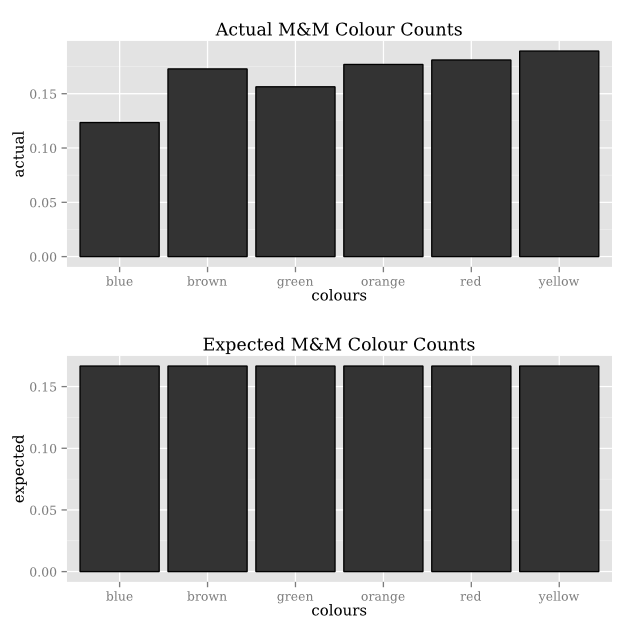
\includegraphics[scale=0.5]{./img/4.png}
            \caption{Observed and Expected M\&M Relative Frequency}
            \label{fig:mnms}
        \end{figure}
    @@ How many blue ones would you expect to see if all colors are equally likely?
    @@@ 200 (Assuming 1200 is the number of M\@Ms in a single bag)
    @@ Do you think your friend is right, based on the one bag evidence? Give a heuristic answer here - you don't need to be precise. What are some of the limitations of this one-bag ``evidence'' approach? In an ideal world, how would you design a study to test this more rigorously?
    @@@ My friend is probably not correct in his assumption. He falls prey to the Texas Sharpshooter Fallacy, which indicates that he only stresses positively affecting results, and downplays negative ones. Using this method is imprecise due to the imperfections that exist in a large enough population. In order to correct this study (and approach it in a more rigorous fashion) I would acquire at minimum 10 bags (probably closer to 1000) and analyze the data over all bags.

    @ The dataset (sample size=40) is given to you for further analysis.
    @@ Plot a default histogram in your favorite software package/program. How many bins does it plot by default for this dataset? What is the size of each bin?
    @@@ Please reference Figure~\ref{fig:default}
        \begin{figure}[!ht]
            \centering
            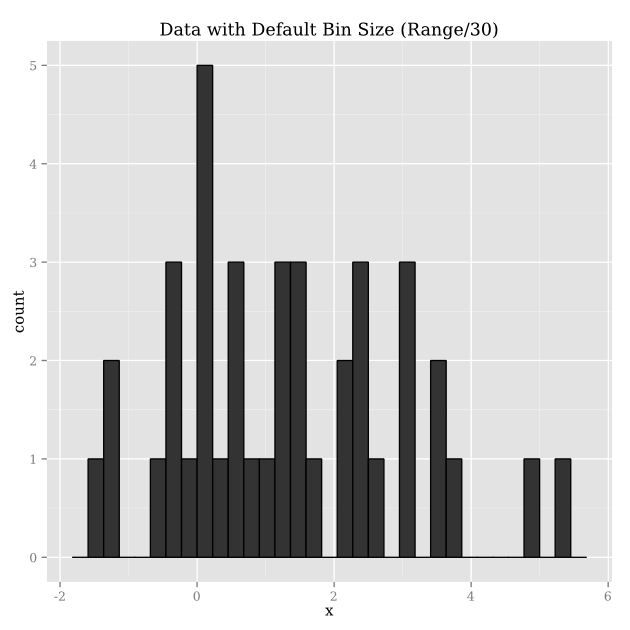
\includegraphics[scale=0.5]{./img/5a.png}
            \caption{Default Bins}
            \label{fig:default}
        \end{figure}
    @@ Change the number of bins - first use 10, then 20, and finally 25. What differences (if any) can you see between these histograms and your histogram from part (a)?
    @@@ Please reference Figure~\ref{fig:bins}
        \begin{figure}[!ht]
            \centering
            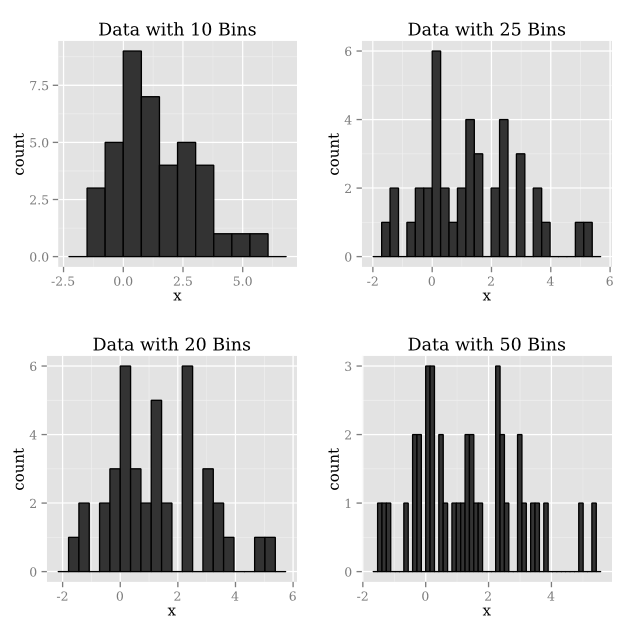
\includegraphics[scale=0.5]{./img/5b.png}
            \caption{Varying Bins}
            \label{fig:bins}
        \end{figure}
    @@ Change the starting point to -2, -1.5, and then -1.45 - and plot a histogram with 25 bins for each.  What differences do you see?
    @@@ Please reference Figure~\ref{fig:index}
        \begin{figure}[!ht]
            \centering
            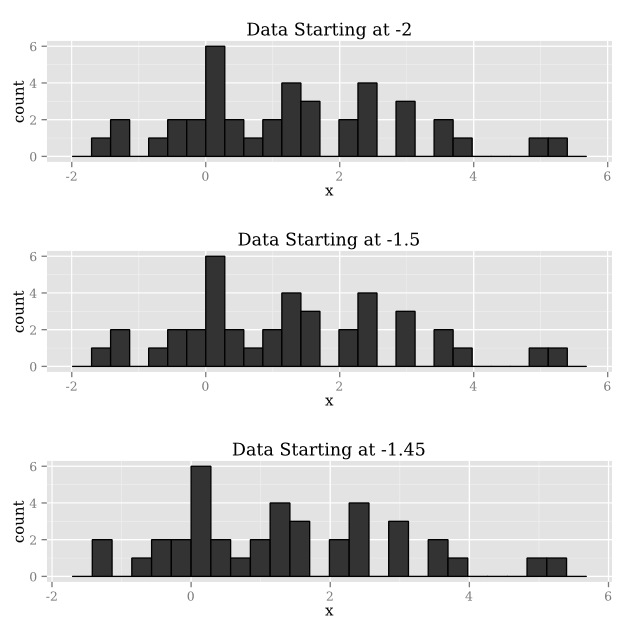
\includegraphics[scale=0.5]{./img/5c.png}
            \caption{Varying Start Index}
            \label{fig:index}
        \end{figure}
\end{easylist}
\end{document}
